\documentclass[a4paper,12pt]{extarticle}

% Геометрия страницы
\usepackage{geometry}
\geometry{left=2.5cm, right=1.0cm, top=2.0cm, bottom=2.0cm}

% === Для русских букв в xelatex ===
\usepackage{fontspec}
\usepackage{polyglossia}
\setmainlanguage{russian}
\setotherlanguage{english}
\setmainfont{CMU Serif}
% ===============================

% Базовые пакеты
\usepackage{amsmath, amsthm, amssymb, mathtools}
\usepackage{graphicx}
\usepackage{color, xcolor}
\usepackage{float}
\usepackage{caption}
\usepackage{subcaption}
\usepackage{booktabs}
\usepackage{colortbl}
\usepackage{tikz}
\usepackage{pgf}
\usepackage{fancyhdr}
\usepackage{setspace}
\usepackage{indentfirst}

% Гиперссылки
\usepackage[colorlinks,
    citecolor=blue,
    linkcolor=blue,
    urlcolor=blue,
    bookmarks=false,
    hypertexnames=true]{hyperref}

% Библиография
\usepackage[
    backend=biber,
    style=numeric,
    maxbibnames=99
]{biblatex}
\addbibresource{refs.bib}

% Таблицы и сноски
\usepackage[flushleft]{threeparttable}
\usepackage{tablefootnote}

% Листинги кода
\usepackage{listings}
\lstset{
    inputencoding=utf8,
    backgroundcolor=\color{gray!10},
    basicstyle=\ttfamily\small,
    keywordstyle=\color{blue}\bfseries,
    language=Python,
    breaklines=true,
    showstringspaces=false,
    frame=none
}

% Вспомогательные настройки
\usepackage{chngcntr}
\counterwithin{table}{section}
\counterwithin{figure}{section}

\setlength{\parindent}{1.25cm}
\renewcommand{\baselinestretch}{1.8}


\usepackage{chngcntr} % нумерация графиков и таблиц по секциям
\counterwithin{table}{section}
\counterwithin{figure}{section}

\graphicspath{{graphics/}}%путь к рисункам

\makeatletter
% \renewcommand{\@biblabel}[1]{#1.} % Заменяем библиографию с квадратных скобок на точку:
\makeatother

\geometry{left=2.5cm}% левое поле
\geometry{right=1.0cm}% правое поле
\geometry{top=2.0cm}% верхнее поле
\geometry{bottom=2.0cm}% нижнее поле
\setlength{\parindent}{1.25cm}
\renewcommand{\baselinestretch}{1.5} % междустрочный интервал


\newcommand{\bibref}[3]{\hyperlink{#1}{#2 (#3)}} % biblabel, authors, year
\addto\captionsrussian{\def\refname{Список литературы (или источников)}}

\renewcommand{\theenumi}{\arabic{enumi}}% Меняем везде перечисления на цифра.цифра
\renewcommand{\labelenumi}{\arabic{enumi}}% Меняем везде перечисления на цифра.цифра
\renewcommand{\theenumii}{.\arabic{enumii}}% Меняем везде перечисления на цифра.цифра
\renewcommand{\labelenumii}{\arabic{enumi}.\arabic{enumii}.}% Меняем везде перечисления на цифра.цифра
\renewcommand{\theenumiii}{.\arabic{enumiii}}% Меняем везде перечисления на цифра.цифра
\renewcommand{\labelenumiii}{\arabic{enumi}.\arabic{enumii}.\arabic{enumiii}.}% Меняем везде перечисления на цифра.цифра

\begin{document}


\newpage
\section*{О чём этот отчёт?}
\vspace{1em}

Настоящий отчёт создан для владельцев заведений общественного питания. Он содержит аналитику отзывов посетителей, собранных с Яндекс.Карт.
Мы используем современные методы обработки естественного языка, чтобы выделить ключевые аспекты в отзывах, определить их настроение (сентимент), а также представить результаты в виде наглядных диаграмм и таблиц.

Цель отчёта — помочь вам лучше понять мнение гостей, определить сильные и слабые стороны заведения и принять обоснованные решения для улучшения качества обслуживания.

\vspace{2em}
Отчёт включает:
\begin{itemize}
    \item распределение отзывов по настроению;
    \item анализ по категориям (еда, обслуживание, атмосфера и т.д.);
    \item распределение звёздных оценок;
    \item тепловые карты и гистограммы;
    \item рекомендации на основе выявленных паттернов.
\end{itemize}

\vspace{1em}
Перейдём к аналитике.

\newpage
\section*{1 Инфографика}
В этом разделе представлены визуальные диаграммы, отражающие ключевые метрики, полученные на основе анализа отзывов.
Они позволяют понять, как гости воспринимают заведение, и что чаще всего упоминается в отзывах.

\subsection*{1.1 О чём чаще всего пишут клиенты}

\begin{figure}[H]
    \centering
        \begin{minipage}{0.48\textwidth}
        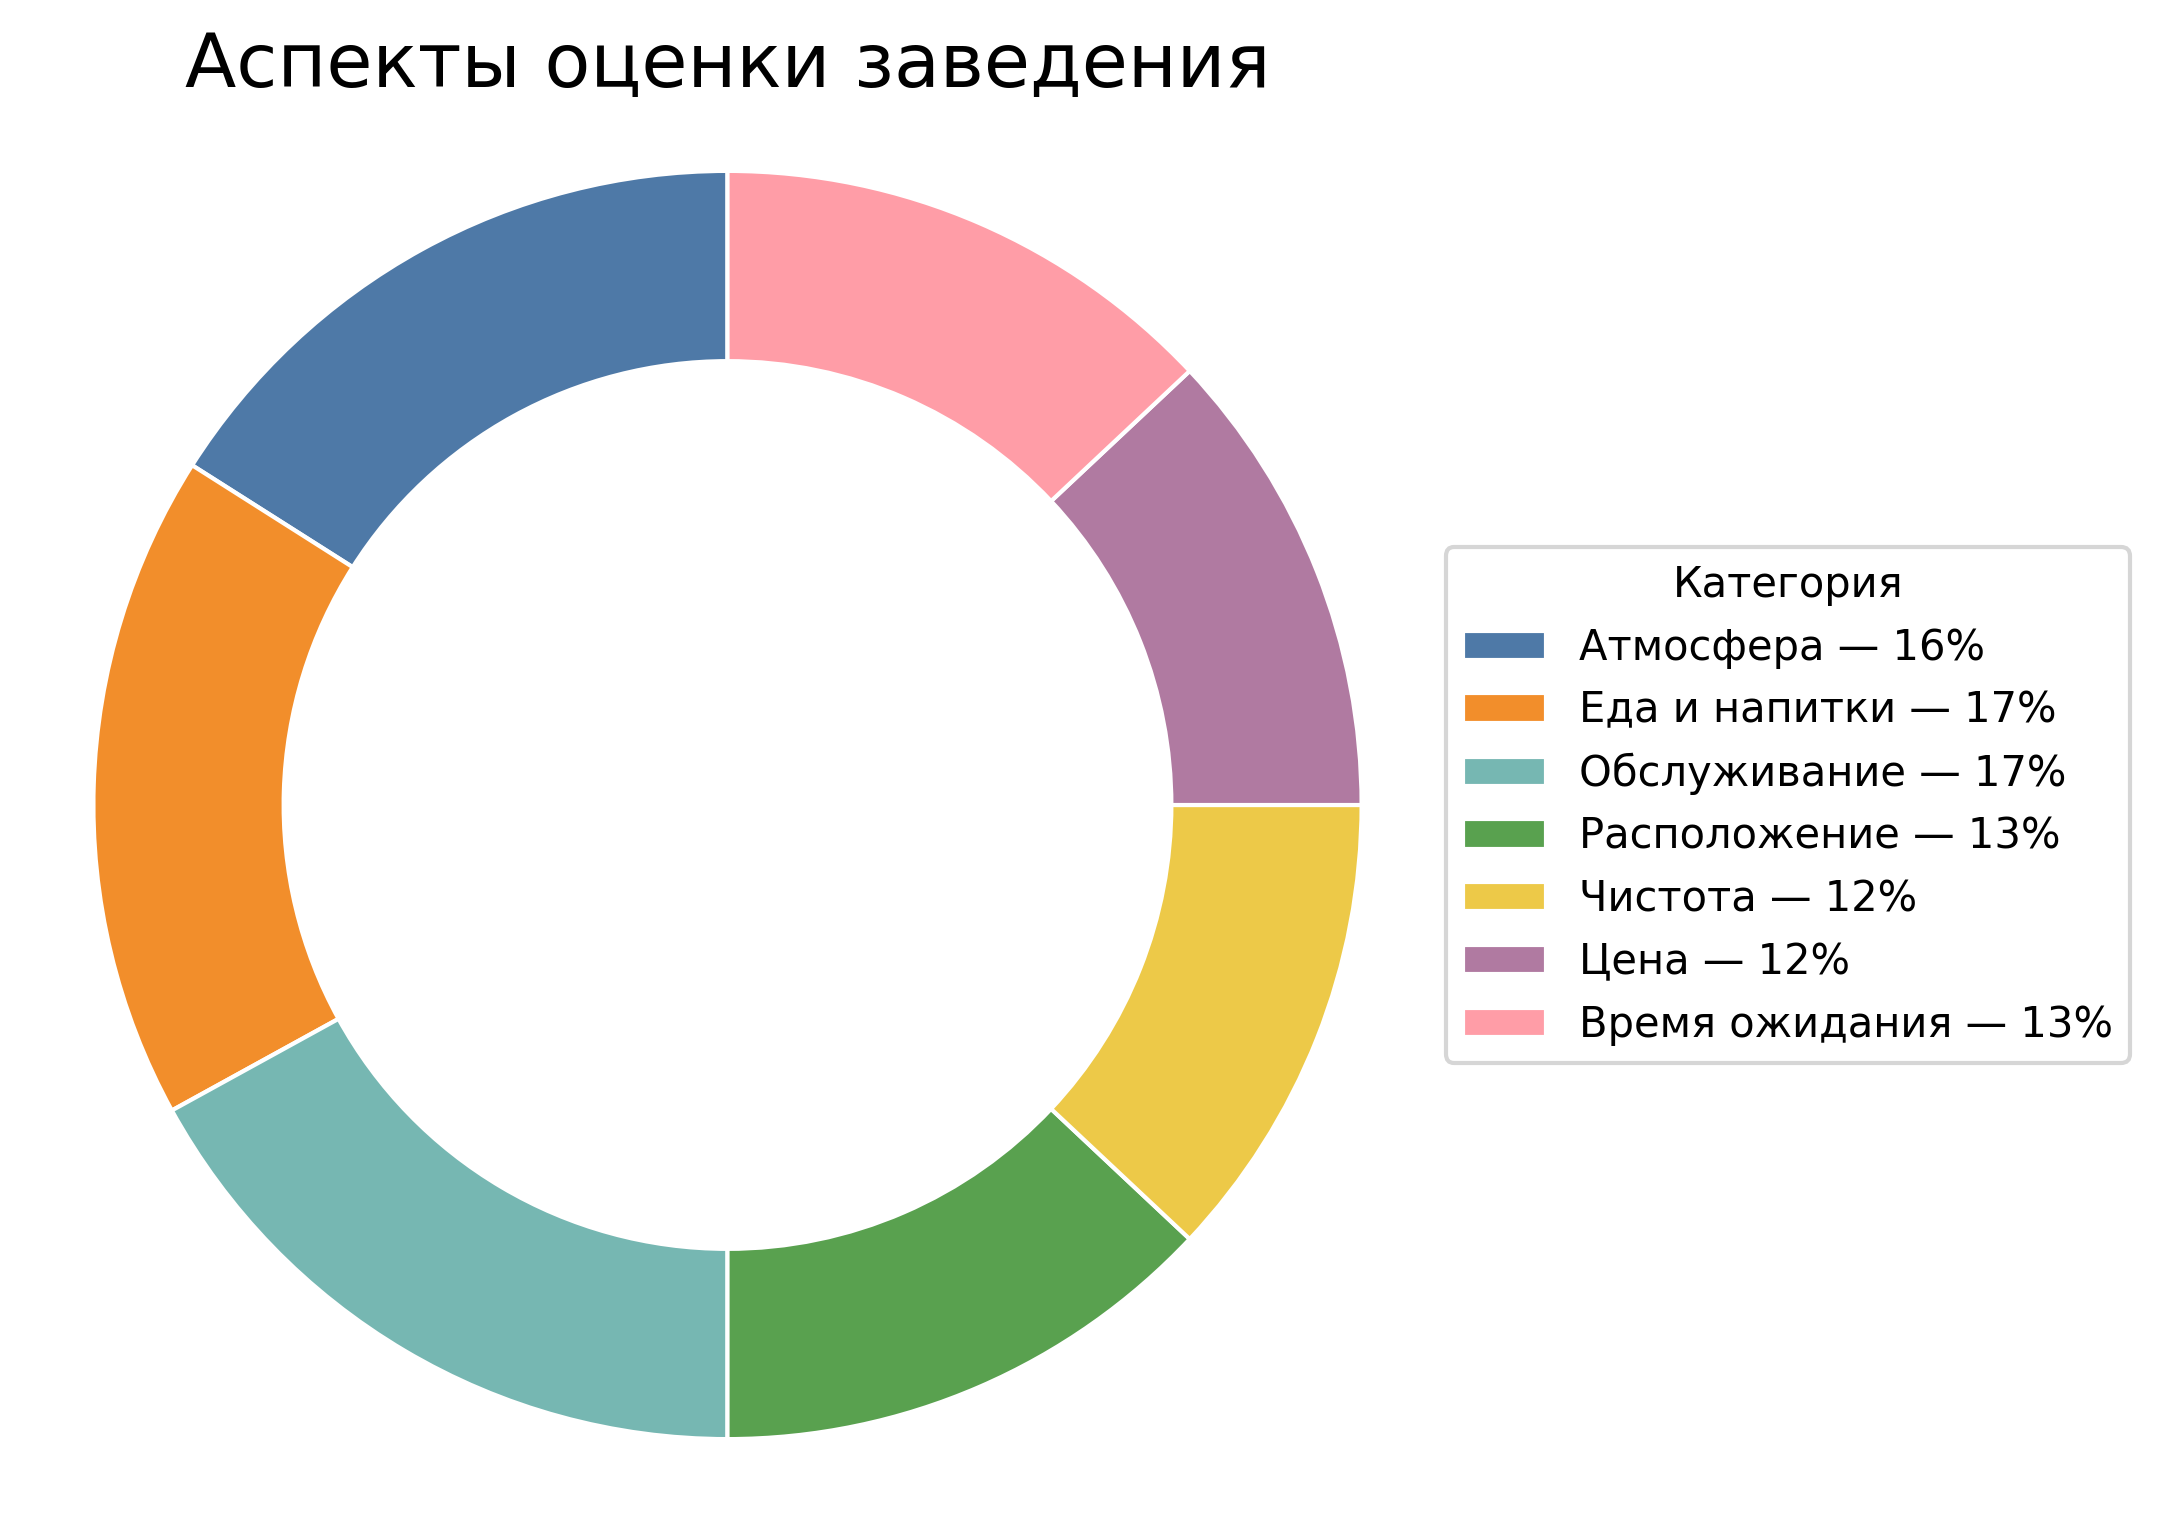
\includegraphics[width=\linewidth]{images/49543885926/category_donut_chart.png}
    \end{minipage}
    \hfill
        \begin{minipage}{0.45\textwidth}
        \small
        \vspace{1em}
    В результате анализа отзывов были выделены 7 ключевых тем, которые чаще всего волнуют гостей при посещении заведения.
    Диаграмма показывает, как часто пользователи упоминали каждую из этих тем. Чем больше доля, тем чаще гости касаются этой категории в своих комментариях.
    \end{minipage}%
\end{figure}

\begin{table}[H]
\centering
\caption*{Основные категории, встречающиеся в отзывах}
\renewcommand{\arraystretch}{1.4}
\begin{tabular}{p{3.5cm}p{12cm}}
\toprule
\textbf{Категория} & \textbf{Описание} \\
\midrule
Атмосфера & Описывает общий уют в заведении: интерьер, оформление, освещение, атмосфера, ощущение комфорта и стиль заведения. \\
Еда и напитки & Все, что касается блюд: вкус, подача, состав, свежесть, разнообразие меню, температура еды и напитков. \\
Обслуживание & Оценка персонала: приветливость, вежливость, ошибки в заказах и скорость реакции на просьбы. \\
Расположение & Удобство добраться до заведения: адрес, близость к транспорту или парковке. \\
Чистота & Состояние зала и санитарных зон: туалеты, столы, посуда, запахи, порядок в зале и на кухне. \\
Цена & Впечатление от стоимости: разумность цен, оправданность по отношению к качеству. \\
Время ожидания & Быстрота обслуживания: скорость подачи блюд и очереди и задержки. \\
\bottomrule
\end{tabular}
\end{table}



\subsection*{1.2 Общнее настроение отзывов}

\begin{figure}[H]
    \centering
    \begin{minipage}{0.48\textwidth}
        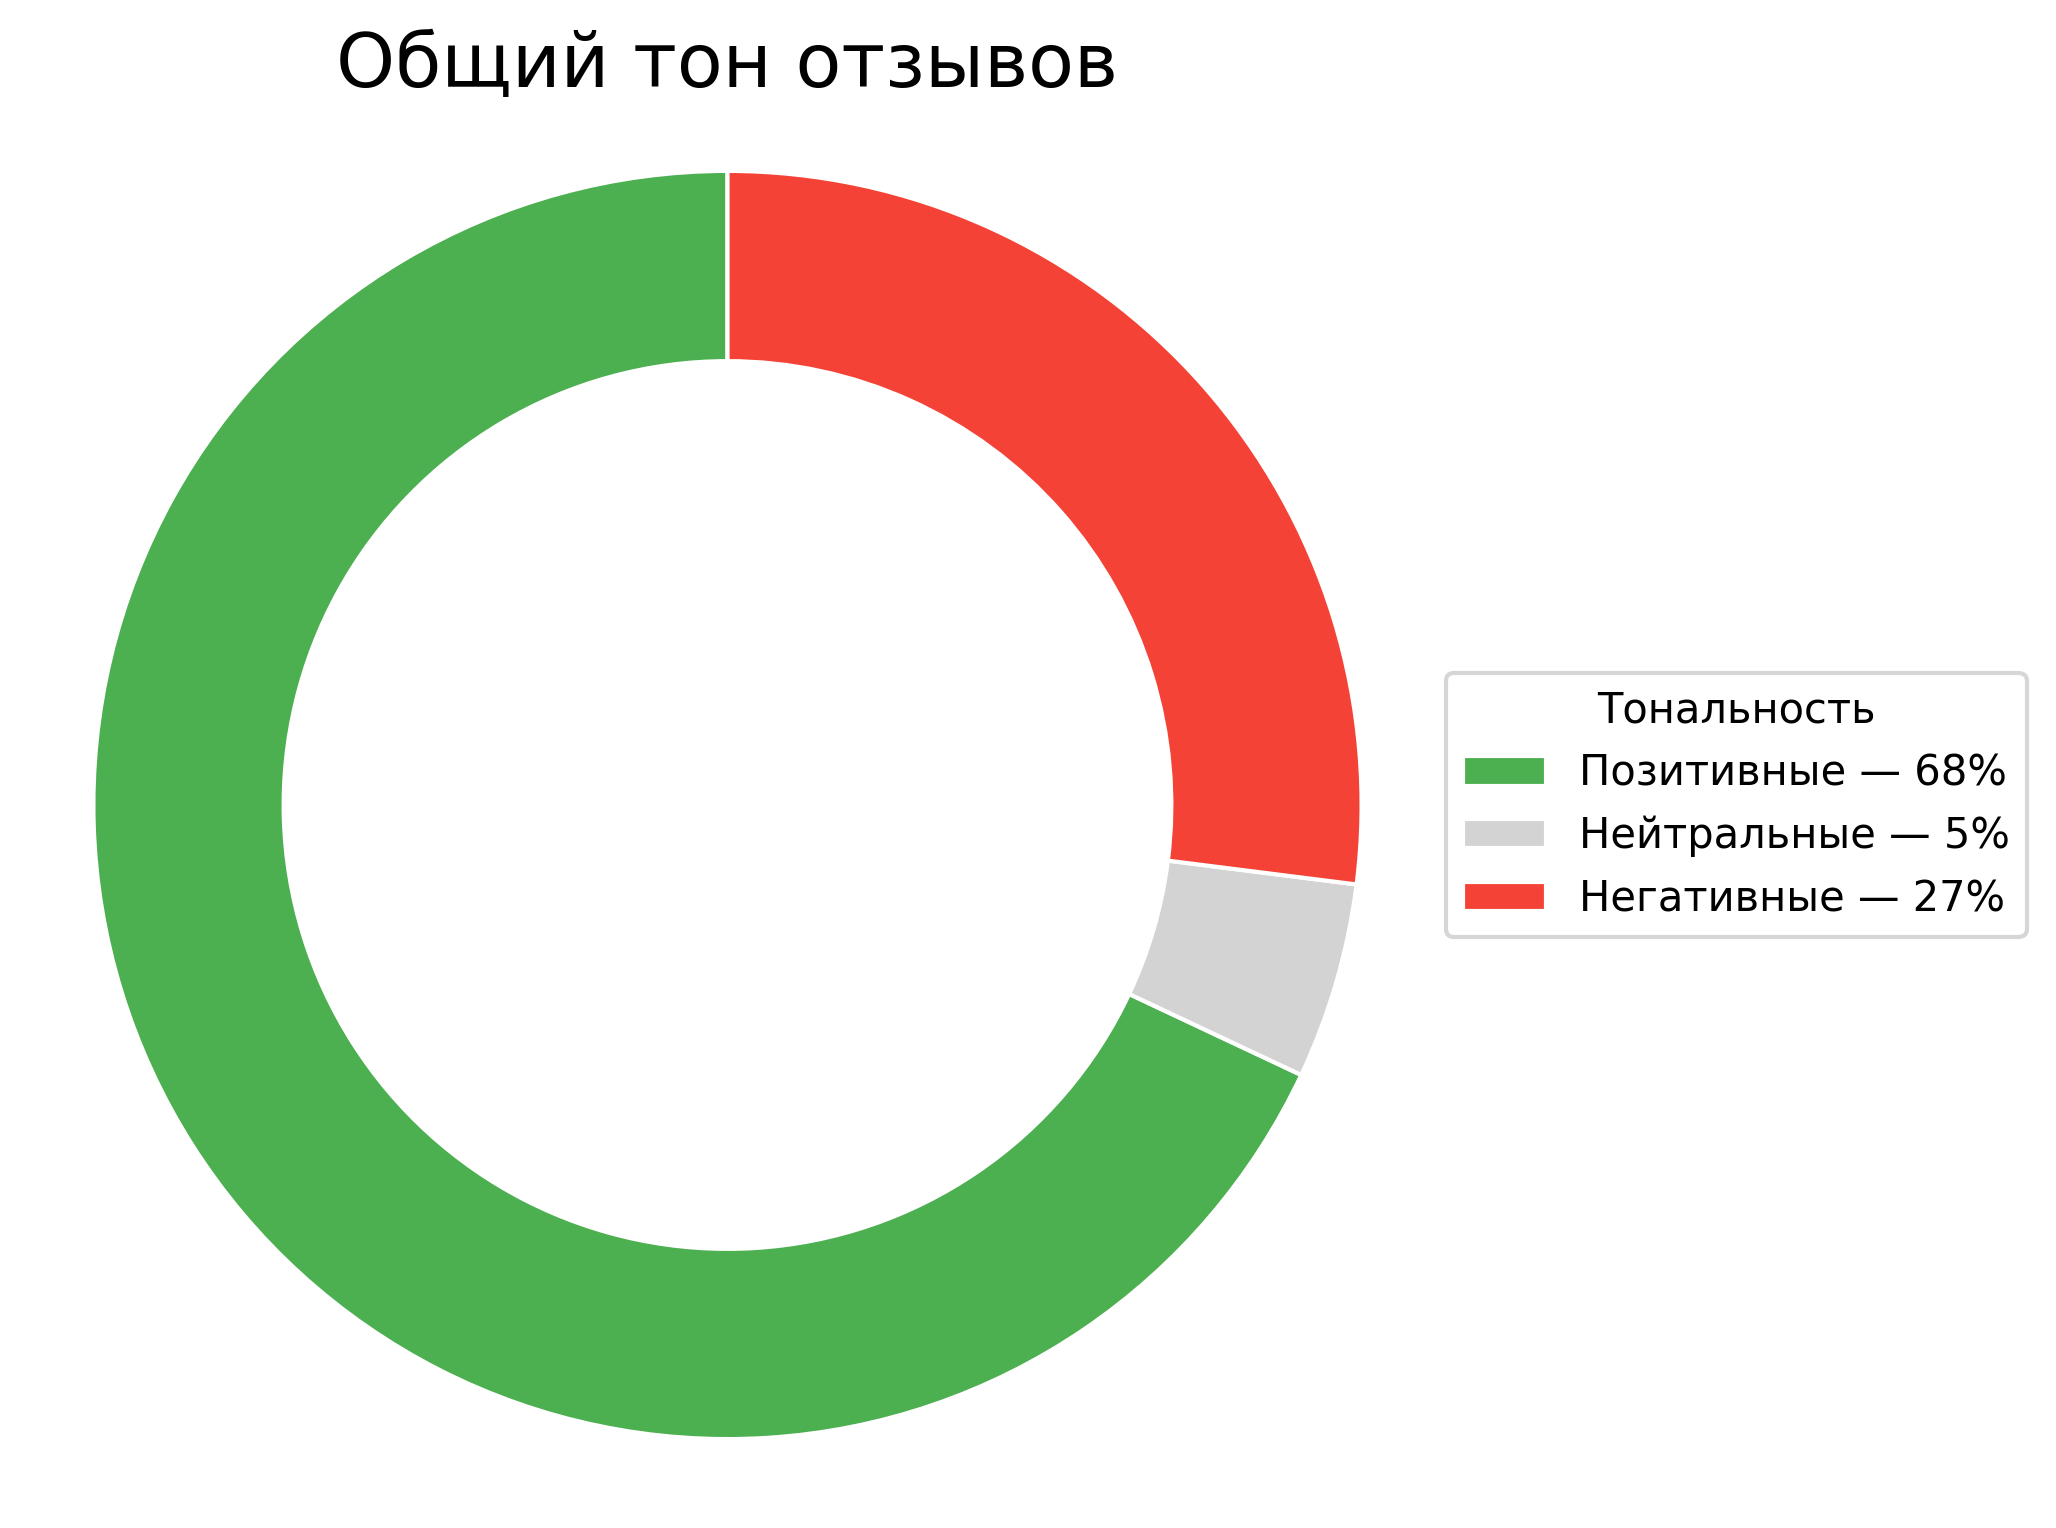
\includegraphics[width=\linewidth]{images/49543885926/sentiment_donut_chart.png}
    \end{minipage}%
    \hfill
    \begin{minipage}{0.48\textwidth}
        \small
        Каждый отзыв, помимо содержания, несёт в себе общее настроение — это называется \textbf{сентимент}.
        \vspace{0.5em}

        Он может быть \textbf{положительным}, \textbf{нейтральным} или \textbf{отрицательным} в зависимости от того, как гость описывает свой опыт.

        \vspace{0.5em}
        Диаграмма справа показывает, сколько отзывов относятся к каждому типу настроения.

        \vspace{0.5em}
        Это позволяет быстро оценить общий эмоциональный фон, с которым клиенты оценивают заведение.
    \end{minipage}
\end{figure}

\subsection*{1.3 Настроение отзывов по темам}
\noindent
Следующий график показывает, как настроение отзывов распределяется по каждой из ключевых категорий.
Это позволяет понять, какие стороны работы заведения воспринимаются положительно, а где гости чаще замечают проблемы или остаются равнодушными.

\vspace{1em}
\begin{center}
    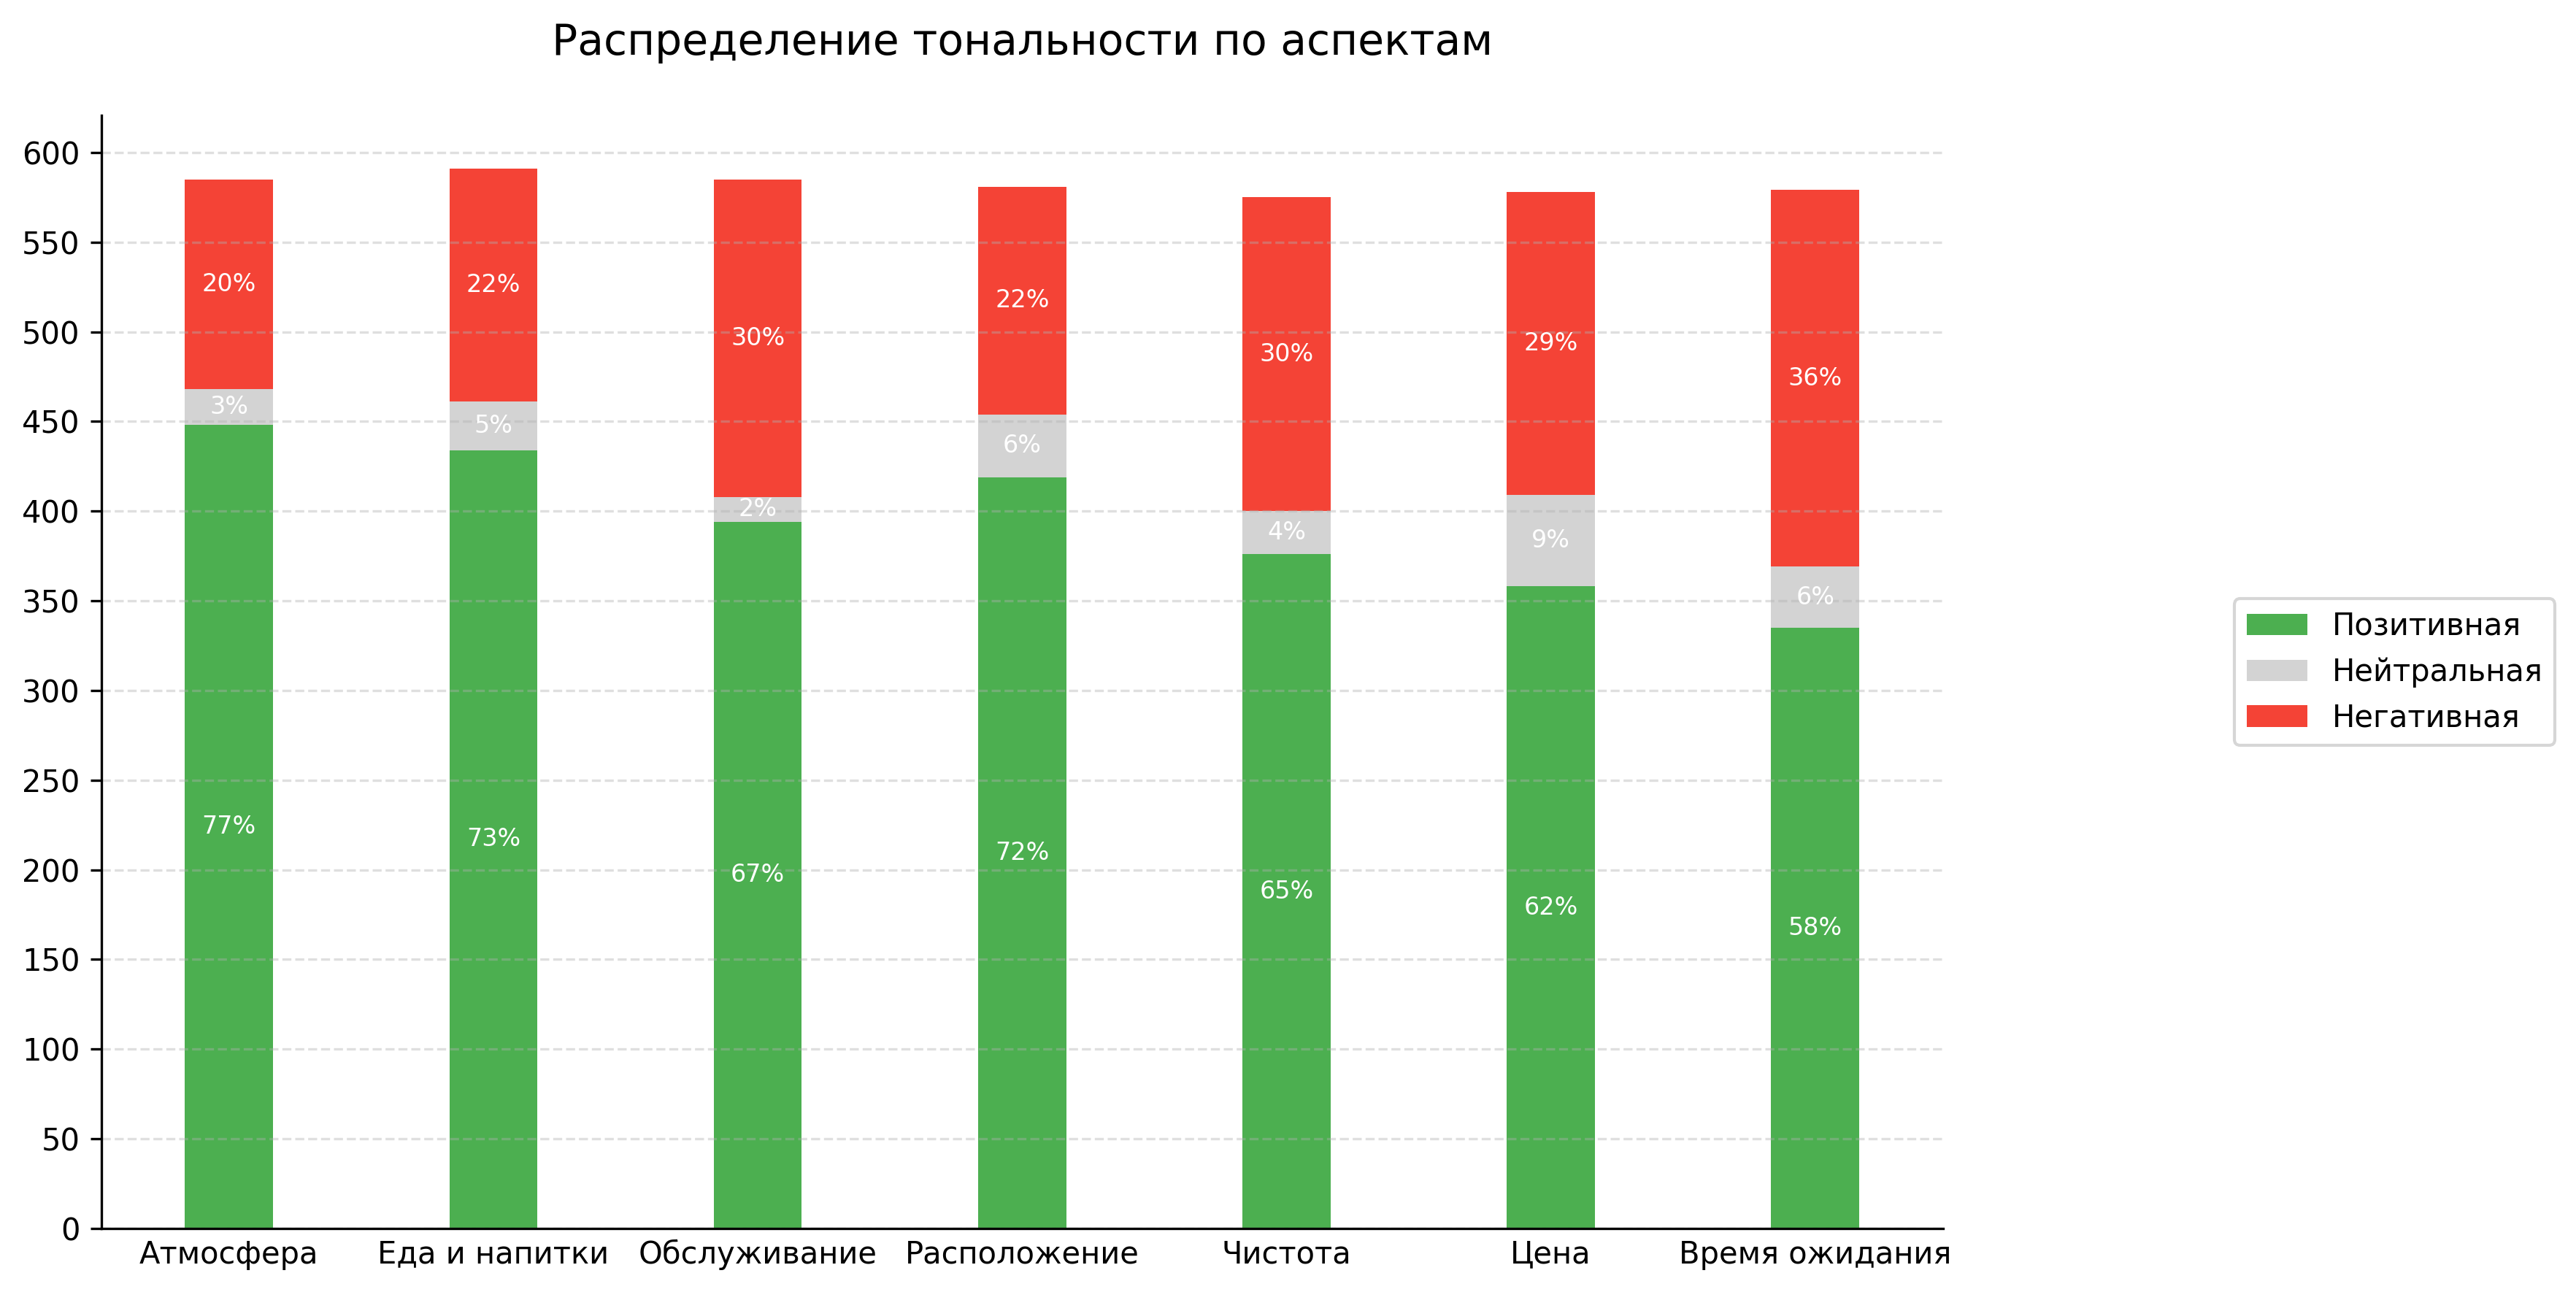
\includegraphics[width=0.95\textwidth]{images/49543885926/histogram.png}
\end{center}
\vspace{1em}

\end{document}